%%% Класс документа
\documentclass[a4paper,14pt]{article}

%%% Работа с русским языком
\usepackage{cmap}					% поиск в PDF
\usepackage[warn]{mathtext}
\usepackage[T2A]{fontenc}			% кодировка
\usepackage[utf8]{inputenc}			% кодировка исходного текста
\usepackage[english,russian]{babel}	% локализация и переносы
\usepackage{mathtext} 				% русские буквы в формулах
\usepackage{csvsimple}              % for tabular from csv loading
\usepackage{indentfirst}            % indent after sections
%\usepackage{minipage}

%%% Дополнительная работа с математикой
\usepackage{amsmath,amsfonts,amssymb,amsthm,mathtools} % AMS
\usepackage{icomma} % "Умная" запятая: $0,2$ --- число, $0, 2$ --- перечисление

%%% Номера формул
%\mathtoolsset{showonlyrefs=true} % Показывать номера только у тех формул, на которые есть \eqref{} в тексте.
%\usepackage{leqno} % Немуреация формул слева

%%% Шрифты
\usepackage{euscript}	 % Шрифт Евклид
\usepackage{mathrsfs}    % Красивый матшрифт

%%% Свои команды
\DeclareMathOperator{\sgn}{\mathop{sgn}}

%%% Перенос знаков в формулах (по Львовскому)
\newcommand*{\hm}[1]{#1\nobreak\discretionary{}
{\hbox{$\mathsurround=0pt #1$}}{}}

%%% Работа с картинками
\usepackage{graphicx}  % Для вставки рисунков
\graphicspath{{images/}{images2/}}  % папки с картинками
\setlength\fboxsep{3pt} % Отступ рамки \fbox{} от рисунка
\setlength\fboxrule{1pt} % Толщина линий рамки \fbox{}
\usepackage{wrapfig} % Обтекание рисунков и таблиц текстом

%%% Работа с таблицами
\usepackage{array,tabularx,tabulary,booktabs} % Дополнительная работа с таблицами
\usepackage{longtable}  % Длинные таблицы
\usepackage{multirow} % Слияние строк в таблице

%%% Теоремы
\theoremstyle{plain} % Это стиль по умолчанию, его можно не переопределять.
%\newtheorem{theorem}{Теорема}[section]
%\newtheorem{proposition}[theorem]{Утверждение}
 
%\theoremstyle{definition} % "Определение"
%\newtheorem{corollary}{Следствие}[theorem]
%\newtheorem{problem}{Задача}[section]
 
%\theoremstyle{remark} % "Примечание"
%\newtheorem*{nonum}{Решение}

%%% Программирование
\usepackage{etoolbox} % логические операторы

%%% Страница
\usepackage{extsizes} % Возможность сделать 14-й шрифт
\usepackage{geometry} % Простой способ задавать поля
	\geometry{top=25mm}
	\geometry{bottom=35mm}
	\geometry{left=35mm}
	\geometry{right=20mm}
	
%%% Колонтитулы
%\usepackage{fancyhdr}
 	%\pagestyle{fancy}
 	%\renewcommand{\headrulewidth}{0mm}  % Толщина линейки, отчеркивающей верхний колонтитул
 	%\lfoot{Нижний левый}
 	%\rfoot{Нижний правый}
 	%\rhead{Верхний правый}
 	%\chead{Верхний в центре}
 	%\lhead{Верхний левый}
 	% \cfoot{Нижний в центре} % По умолчанию здесь номер страницы
 	
%%% Интерлиньяж
%\usepackage{setspace}
%\onehalfspacing % Интерлиньяж 1.5
%\doublespacing % Интерлиньяж 2
%\singlespacing % Интерлиньяж 1

%%% Гиперссылки
\usepackage{hyperref}
\usepackage[usenames,dvipsnames,svgnames,table,rgb]{xcolor}
\hypersetup{				% Гиперссылки
    unicode=true,           % русские буквы в раздела PDF
    pdftitle={Заголовок},   % Заголовок
    pdfauthor={Автор},      % Автор
    pdfsubject={Тема},      % Тема
    pdfcreator={Создатель}, % Создатель
    pdfproducer={Производитель}, % Производитель
    pdfkeywords={keyword1} {key2} {key3}, % Ключевые слова
    colorlinks=true,       	% false: ссылки в рамках; true: цветные ссылки
    linkcolor=red,          % внутренние ссылки
    citecolor=green,        % на библиографию
    filecolor=magenta,      % на файлы
    urlcolor=cyan           % на URL
}

%%% Другие пакеты
\usepackage{lastpage} % Узнать, сколько всего страниц в документе.
\usepackage{soul} % Модификаторы начертания
\usepackage{csquotes} % Еще инструменты для ссылок
%\usepackage[style=authoryear,maxcitenames=2,backend=biber,sorting=nty]{biblatex}
\usepackage{multicol} % Несколько колонок
\usepackage{multirow} % Несколько строк

%%% Шрифты
%\renewcommand{\familydefault}{\sfdefault} % Начертание шрифта


%%% Работа с библиографией
%\usepackage{cite} % Работа с библиографией
%\usepackage[superscript]{cite} % Ссылки в верхних индексах
%\usepackage[nocompress]{cite} % 
%\usepackage{csquotes} % Еще инструменты для ссылок


%%% Tikz
\usepackage{tikz} % Работа с графикой
\usepackage{pgfplots} % Работа с pgf
\usepackage{pgfplotstable}
\usepackage{upgreek}

%%% Дополнительные пакеты для tikz
%\usepgfplotslibrary{dateplot} % Возможность подписания дат
\pgfplotsset{compat=1.5}

\author{Филиппенко Павел, Сибгатуллин Булат}
\title{Верстка научных отчетов в \LaTeX{}}
\date{\today}

\begin{document}
    %% сделать красивый титульник
    \maketitle
    \thispagestyle{empty}

    \newpage
    \tableofcontents{} %содержание
    \newpage

    \section{\LaTeX{} что это такое?}

    \subsection{Введение}

    Любую лабораторную работу или научную статью важно не только сделать правильно и грамотно, но и добиться того, чтобы она была презентабильной и хорошо выглядела. В этом нам поможет культовая среда для верстки \LaTeX{}.
    %% вставить эмблему латеха
    Для оформления лабораторных работ или иных документов многие используют Word или LibreOffice Writer. Однако обе эти программы имеют ряд недостатков и в вопросе верстки научного текста значительно уступают \LaTeX{}.

    Что такое \LaTeX{}?  
    Согласно Википедии: \LaTeX{} -- наиболее популярный набор макрорасширений (или макропакет) системы компьютерной вёрстки \TeX, который облегчает набор сложных документов. Пакет позволяет автоматизировать многие задачи набора текста и подготовки статей, включая набор текста на нескольких языках, нумерацию разделов и формул, перекрёстные ссылки, размещение иллюстраций и таблиц на странице, ведение библиографии и др.
    Возможно данное определение звучит несколько сложновато. Не забивая голову лишним, можете считать \LaTeX инструментом оформления научных отчетов. Более глубокое понимание придет с практикой.

    \begin{figure}[h!]
        \centering
        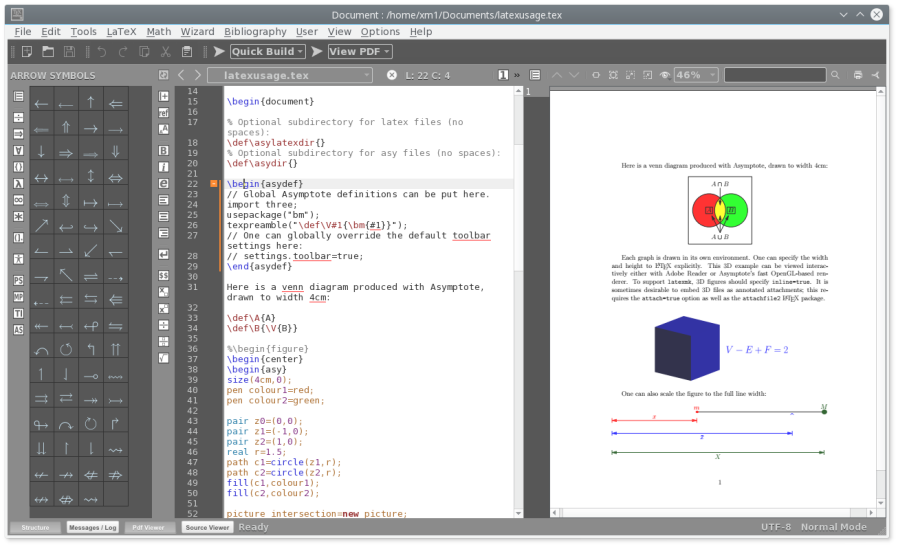
\includegraphics[width = \textwidth]{TexCode_example.png}
        \caption{}
        % \label{}
    \end{figure}

    \newpage

    \subsection{Преимущества \LaTeX}

    Чем же так хорош \LaTeX? В целом можно выделить 4 основных преимущества

    \begin{enumerate}
        \item Подгоняет документ ко всем типографским стандартам. Таким образом, можно полностю сконцентрироваться на содержании документа, а не на его оформлении.
        \item Автоматизация процессов: автоматическая нумерация разделов и формул, автоматическое составление оглавления и многое другое. Меньше рутины.
        \item Открытая среда. Обширное community. В интернете можно найти ответы на любые ваши вопросы, большое количество информации, а так же пакетов, расширений и фич.
        \item Кроссплатформенность.
    \end{enumerate}

    \subsection{Как оно работает???}

    В некотором смысле работа \LaTeX похожа на известные вам языки программирования. На вход подается исходный код, затем происходит компиляция и на выходе мы получаем тепленький красивый pdf-документ.

    %% картинки исходного кода и готового документа

    \section{Редакторы кода}

    Для работы с \LaTeX необходимо 2 вещи: специальный компилятор, который будет магическим образом превращать ваши исходники в pfd и редактор кода, в котором вы будете непосредственно работать.
    
    \begin{wrapfigure}{l}{0.25\textwidth}
        \centering
        
\includegraphics[width = 0.2\textwidth]{texmaker220-220.jpg}
        \caption{}
        %\label{fig:}
    \end{wrapfigure}

    Существует большое количество программ, которые представляют собой визуальную графическую среду для создания и редактирования документов \LaTeX.
    Наиболее распространенным вариантом являются программы TexMaker и TexStudio. Это кросс-платформенные редакторы \LaTeX с открытым кодом. Данные программы являются интегрированными средами для создания \LaTeX документов и включают такие возможности, как интерактивная система проверки правописания, сворачивание блоков текста, подсветка синтаксиса и многое другое.

    \begin{wrapfigure}{r}{0.25\textwidth}
        \centering
        
\includegraphics[width = 0.2\textwidth]{Texstudio_Logo.png}
        \caption{}
        %\label{fig:}
    \end{wrapfigure}

    % фотографи TexMaker и TexStudio

    %% Пара слов про VS-Code

    Мы же будем использовать веб-редактор латех документов OverLeaf. Его основное преимущество заключается в том, что данный редактор не требует никакой установки, воспользоваться им можно с любой платформы на любом устройстве с выходом в интернет.
    Кроме того, этот редактор позволяет нескольким пользователям редактировать один и тот же документ одновременно и просматривать изменения друг друга в режиме реального времени.

    \begin{figure}[h!]
        \centering
        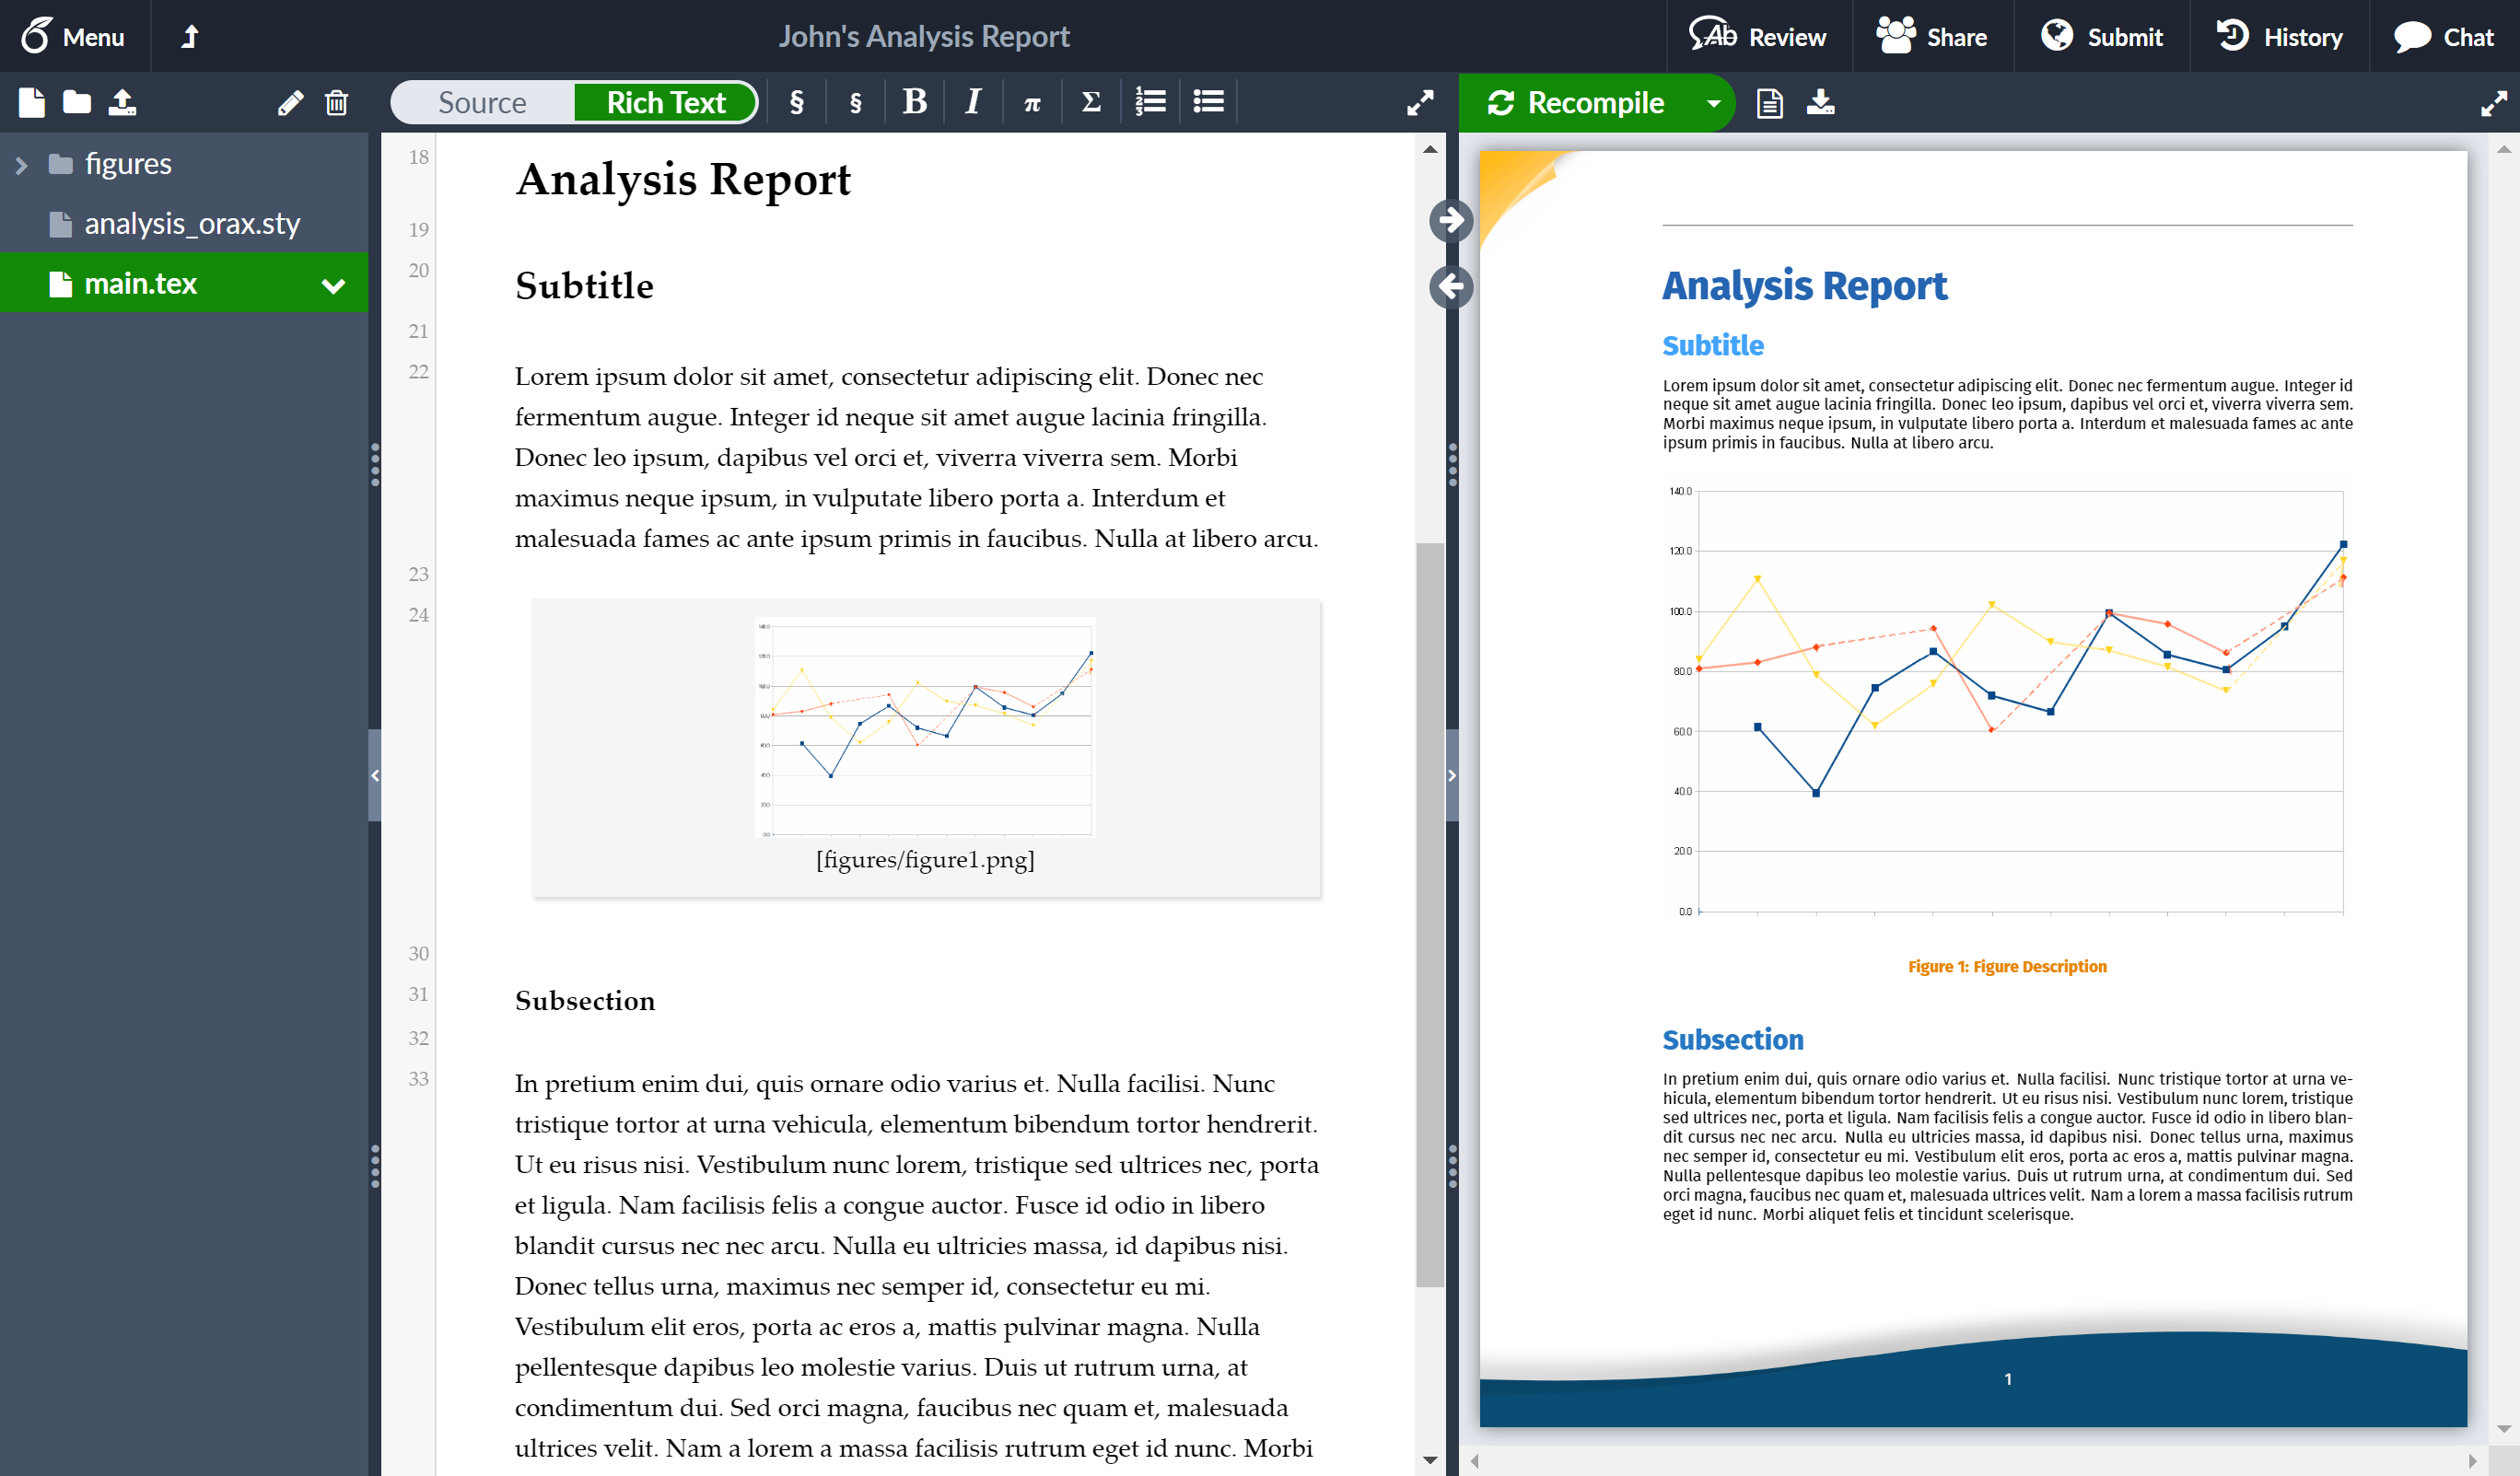
\includegraphics[width=\linewidth]{OverLeaf_example.png}
        \caption{}
        \label{OverLeaf_example}
    \end{figure}

    \section{Overleaf}

    \subsection{Регистрация}

    Давайте же познакомимся с нашим текстовым редактором. Для этого перейдем на сайт 
    %%\href{https://www.overleaf.com/login}{https://www.overleaf.com/login} 
    https://www.overleaf.com/login и сразу попадем на страницу регистрации. 

    %% input a beautiful instruction pictures
    
    Чтобы зарегистрироваться, необходимо внизу экрана выбрать пункт Register.

    %% input a beautiful instruction pictures

    Вводим адрес электронной почты и придумываем пароль. После этого на вам предложат создать ваш первый проект, а на почту придет письмо с просьбой подтвердить адрес. Абсолютно ничего сложного,
    подтверждаем адрес и создаем наш первый проект Blank Project.

    %% input a beautiful instruction pictures

    \subsection{Знакомство с интерфейсом}

    \section{Начало работы}
    \section{Математика}
    \section{Рисунки и таблицы}
    \section{Ссылки}
\end{document}